\documentclass{article}
\usepackage{amsmath,amssymb}
\usepackage[a4paper,textwidth=450pt]{geometry}
\DeclareMathOperator{\E}{\mathbb{E}}
\usepackage[utf8]{inputenc}
\usepackage[english]{babel}
\usepackage{biblatex}
\addbibresource{novel.bib}
\usepackage{graphicx}
\usepackage{indentfirst}
\usepackage{physics}
\usepackage{refcheck}
\usepackage{units}
\usepackage{wrapfig}
\usepackage{subcaption}
\usepackage{booktabs}
\usepackage{multirow}
\usepackage{graphicx}
\usepackage{csquotes}
\setkeys{Gin}{width=.6\textwidth}
% !TeX spellcheck = en_GB
\graphicspath{ {./images/} }

\newtheorem{proposition}{Proposition}

\newenvironment{proof}
 {\begin{trivlist} \item[] {\bf Proof.\ }}{\hfill$\Box$ \end{trivlist}}

\title{Newsvendor Problems: A New Integrated Approach\\ to Forecasting and Optimisation}

\author{Congzheng Liu\thanks{Department of Management Science,
Lancaster University, Lancaster LA1 4YX, UK.
Email: {\tt \{c.liu19,a.n.letchford,i.svetunkov\}@lancaster.ac.uk}}
\and Adam N.\ Letchford$^*$ \and Ivan Svetunkov$^*$} % end author list

\date{Draft, 27th July 2020}

\begin{document}

\maketitle

\begin{abstract}
Newsvendor problems form a classical and important family of stochastic optimisation problems. The standard solution approach decomposes the problem into two steps: estimation of the demand distribution, then determination of the optimal production quantity (or quantities) for the given distribution. We propose a new, integrated solution approach, which estimates the optimal production quantity directly from the data. We conduct simulations in order to show that the proposed approach performs similar to the conventional ones on the well-behaved data if the forecasting model is correctly specified and outperforms the others, when the wrong model is applied to the data. It also demonstrates advantages, when applied to the nonlinear newsvendor problem.% Our approach can be used even when the demand distribution is not stationary. Some encouraging computational results are given. 
\\*[2mm]
{\bf Keywords:} newsvendor problems, forecasting, data-driven optimisation, sales and operations planning
\end{abstract}


%%%%%%%%%%%%%%%%%%%%%%%%%%%%%%
\section{Introduction}

Inventory control is a classical and important topic in Operations Research and Operations Management (see, e.g., the books \cite{Po02,SPP98,Zi00}). In this paper, we focus on \emph{Newsvendor Problem} (NVP), which refers to a \emph{single-period} \emph{stochastic} inventory control problem.

In early works on NVP \cite{AHM51,MK51}, it is assumed that the demand in each time period comes from a known probability distribution. Of course, in practice, this is not the case --- a fact already noted in 1958 by Scarf \cite{Sc58}. Assuming that historical demand data is available, one can attempt to address this issue by decomposing the problem into an estimation / forecasting and an optimisation phases.
In the first phase, one makes some assumptions (e.g., normality) regarding the underlying data generating process, and uses the past data to estimate the parameters of the model.
In the second phase, one determines the order quantity (or quantities) based on the estimated parameter values.

Throughout this paper, we will call this two-phase approach the \emph{disjoint} approach. An advantage of the disjoint approach is that forecasting and optimisation experts can operate independently within an organisation. This makes things easier to manage. On the other hand, as noticed by several authors \cite{BT06,BM12,Ka94,KT96,KTB20}, there are two disadvantages:
\begin{itemize}
\item The two phases use different objective functions. Indeed, in the first phase, the objective is to minimise a function of the forecasting errors, such as the root mean square error or mean absolute error. In the second phase, however, the goal is usually to maximise expected profit.
\item If the forecasting model is misspecified, and/or there is substantial noise in the data, the effect on the optimisation phase is very hard to predict. In particular, upside and downside errors may have very different effects on expected profit, due to different overage/underage cost.
\end{itemize}

An alternative to the disjoint approach is to use a single, \textit{integrated} approach, in which the order quantities are determined directly from the data. A simple example of an integrated approach is \emph{quantile regression} \cite{Br16,Hu19}, which does not make assumptions about the demand distribution. Unfortunately, it can only be applied to relatively simple NVPs, for which one can express the optimal order quantities in terms of quantiles of demand.

In this paper, we introduce a new integrated approach. It is very flexible, and can be applied to a wide variety of NVPs, with complex profit functions. Roughly speaking, it involves forecasting the optimal order quantities instead of the demand, which is done via the maximisation of the expected profit instead of estimating parameters via the minimisation of a function of forecast errors.

We demonstrate in this paper that the proposed approach reduces to quantile regression in the case of the simplest NVP. We then perform extensive computational experiments, on several different NVPs, the results of which show that our method performs at least as good as the disjoint approach, according to several different measures of quality.

The rest of the paper is organised as follows. Section \ref{se:lit} provides a brief review of the relevant literature. Section \ref{se:new} presents the new method and shows that it is a generalisation of quantile regression. In Section \ref{se:results}, we present and discuss the computational results. Finally, Section \ref{se:end} gives some insights, remarks and suggestions.

%%%%%%%%%%%%%%%%%%%%%%%%%%%%%%
\section{Literature Review} \label{se:lit}

Since the literature on NVPs is vast, we mention here only works of direct relevance. The reader looking for more information is directed to the books on the subject \cite{Ch12,Po02,SPP98,Zi00}.

\subsection{The classical newsvendor problem} %\label{sub:lit1}

In the simplest NVP, found in textbooks \cite{Ch12}, a company purchases goods at the beginning of a time period at a cost of $v$ per unit, and aims to sell them by the end of the period at a price $p$ per unit. The demand during the period is a random variable $Y$ with known probability density function $f$ and cumulative distribution function $F$. At the end of the period, any surplus goods will lead to a \emph{holding cost} of $c_h$ per unit. On the other hand, shortage of goods during the period will lead to a \emph{shortage cost} of $c_s$ per unit. The goal is to determine an \emph{order quantity} $Q$, prior to the period, that maximises the expected profit.

For a given $Q$ and a given realisation $y$ of $Y$, the profit over the period is:
\[
    \pi(Q,y)=
    \begin{cases}
        py-vQ-c_h(Q-y),& \text{if } Q\geq y\\
        pQ-vQ-c_s(y-Q),& \text{if } Q< y.
    \end{cases}
\]
The expected value of $\pi(Q,y)$ is:
\[
    \Pi(Q) = \int_{0}^{Q} \big[ py-vQ-c_h(Q-y) \big] f(y)dy + \int_{Q}^{\infty} \big[ pQ-vQ-c_s(y-Q) \big] f(y)dy.
\]

It is common to call $c_u= p-v+c_s$ the ‘underage’ cost and $c_o = v+c_h$ the ‘overage’ cost. Some calculus then shows that the order quantity that maximises $\Pi(Q)$ is \cite{Ch12}:
\[
    Q^* = F^{-1}\left( \frac{c_u}{c_o+c_u} \right),
\]
where $F^{-1}$ is the inverse function of $F$. Thus, $Q^*$ is the $\tau$\textsuperscript{th} quantile of $f$, with $\tau=\nicefrac{c_u}{(c_o+c_u)}$. One can think of the quantity
$c_u/(c_o+c_u)$ as a ``target service level", since that aiming for this target will bring the company maximised expected profit.

\subsection{More complex newsvendor problems} %\label{sub:lit2}

Since the introduction of NVP in the 1950s \cite{AHM51,MK51}, researchers have considered several extensions of the problem, including variants with multiple product types \cite{HW63,LL96,MS00}, quantity discounts \cite{Kh95}, different risk measures \cite{EGS95}, product substitution \cite{BAA99}, nonlinear cost functions \cite{HOS12}, non-stationary demand \cite{KWH15}, and price setting \cite{KC62,Mi59,PD99}.

For the purpose of what follows, we now explain one variant, the `Nonlinear Newsvendor Problem' (NNV), in detail (see also \cite{BT06,HOS12,HN16,KC62,Kh95,KK18,Mi59,PSC15,PD99,Por02,Por90}). In the NNV, the profit function takes the form:
\[
    \pi(Q,y)=
    \begin{cases}
        P(Q,y)-V(Q)-C_h(Q,y),& \text{for } Q \geq y\\
        P(Q,y)-V(Q)-C_s(Q,y),& \text{for } Q< y,
    \end{cases}
\]
where $V$, $P$, $C_h$ and $C_s$ are now \emph{functions} rather than constants.

If $\pi(Q,y)$ has a particularly simple form (e.g., if it is piecewise-linear as in classical NVP), then it may be possible to  use calculus to express the optimal order quantity as a quantile \cite{Ch12}. In general, however, a closed-form expression as a quantile is unlikely to exist \cite{HOS12,Por02,Por02}.

We now review one particular example of NNV, taken from \cite{KK18,PD99,RK02}, that we are going to use in our numerical experiments. The purchase cost $v$ and selling price $p$ are fixed, but $C_h$ and $C_s$ are functions. Overstock items incur a constant unit penalty $\alpha > 0$, but they can be sold in a salvage market with fixed unit sales price $\beta$, with $0<\beta<v$. The demand in the salvage market is itself a random variable, with known distribution, which we denote by $u$. That is, we have:
\[
    C_h(Q,y) \, = \, \alpha[Q-y]^{+} - \beta \E \Big[ \min \big\{ [Q-y]^{+},u \big\} \Big].
\]
Moreover, the shortage penalty is proportional to the shortage quantity. That is:
\[
C_s(Q,y) =  \zeta \, \big( [y-Q]^{+} \big)^2
\]
for some constant $\zeta > 0$. Approximation method and solution can be found in \cite{KK18}.

\subsection{Quantile regression} \label{sub:lit3}

Returning to the classical NVP, we now consider the (more realistic) case in which the demand distribution is unknown, but we have historical demands $y_1,y_2,\dots,y_s$.
For this case, \emph{quantile regression}
has proven to perform well, and the basic idea is as follows \cite{BT06,Br16,CS19,HNS15,Hu19}:
\begin{enumerate}
\item Compute the value of $\tau$ that maximises expected profit;
\item Use quantile regression to compute an estimate of the $\tau$\textsuperscript{th} quantile of the demand in the next time period, which we denote by $\hat{y}_{s+1}^{(\tau)}$;
\item Set the order quantity $\hat{Q}_{s+1}$ to $\hat{y}_{s+1}^{(\tau)}$.
\end{enumerate}

The biggest advantage of quantile regression is that this method doesn't require the assumption of a specific demand distribution \cite{Hu19}. However, it is efficient only on large samples \cite{Hu19,RV19}. Another drawback is that the performance of this approach depends crucially on the underlying target service level. Huber \cite{Hu19} and Rudin \cite{RV19} demonstrated that the benefit of using the quantile regression method is limited to target service levels smaller than 0.8. If the target service level is higher, then much more data is needed in order to correctly estimate specific quantile.

While quantile regression can be used efficiently for the classical NVP given enough historical data, it fails in case of NNV when there doesn't exist a closed-form solution. This is because the specific demand quantiles do not necessarily propagate correctly to the correct orders.

\subsection{Other integrated approaches} %\label{sub:lit4}

There exist other integrated methods. One approach is to use machine learning techniques, such as neural networks, to estimate the optimal order quantity from historical data. The application of machine learning to NVPs can be seen in \cite{CS19,OST20,RV19}. Another integrated approach is based on so-called \emph{one-shot decision theory} \cite{Guo11,GM14,Ma19}. A numerical example was shown in \cite{Guo11}, and extensions can be found in \cite{Ma19}. For the sake of brevity, we do not describe these alternative integrated methods in detail.

%%%%%%%%%%%%%%%%%%%%%%%%%%%%%
\section{The Proposed Estimator for NVPs} \label{se:new}

%We have seen that, while quantile regression can be an attractive integrated approach, it has some drawbacks. In particular, for most non-trivial NVPs, it is very hard to express the optimal order quantity as a demand quantile \emph{a priori}.
In order to overcome the limitations of quantile regression, we propose an alternative integrated method, based on a regression model with a specialised loss function.

For each historical period $t\in [1,s]$, we assume that the observed demand $y_t$ is a realisation of a random variable $Y_t$. Then, in principle, there exists an order quantity, say $Q_t^*$, that maximises the expected profit given $Y_t$ and $\Pi$. Thus, if we had set $Q_t$ to $Q_t^*$ prior to observing the true demand $y_t$, we would have maximised our expected profit in period $t$. Putting it another way, if we could somehow uncover the structure of the unobservable time series $\big\{ Q_1^*,\dots,Q_s^* \big\}$, we would be able to estimate $Q_{s+1}^*$ directly.

Of course, in practice, the distribution of $Y_t$ is unknown, and the values $Q_t^*$ are not observable. So we approximate the $Q_t^*$ values using a linear regression model. For each $t$, the regression model yields an estimate of $Q^*_t$, which we denote by $\hat{Q}_t$. The estimate $\hat{Q}_{s+1}$ can then be used as the order quantity in the next time period.

The crucial feature of our approach is that, instead of using the standard loss functions (such as least squares or maximum likelihood) to estimates the regression parameters, we find the parameters that maximise the empirical expected profit function $\sum_{t=1}^s{\pi \big( \hat{Q}_t,y_t \big)}$. This can be expressed as:
\[
    \hat{\boldsymbol{\beta}}=\text{argmax}_{\boldsymbol{\beta}\in \mathbb{R}^{p+1}}\displaystyle\sum_{t=1}^s{\pi(\hat{Q}_t,y_t)},
\]
based on the assumption of a linear relationship of the form
\[
    \mathbf{\hat{Q}}=\mathbf{X}\boldsymbol{\beta},
\]
where
\[
    \mathbf{\hat{Q}}=
    \begin{pmatrix}
        \hat{Q}_1\\
        \hat{Q}_2\\
        \vdots\\
        \hat{Q}_s
    \end{pmatrix}, \quad
    \mathbf{X}=
    \begin{pmatrix}
        \mathbf{x}_1^{\mathsf{T}}\\
        \mathbf{x}_2^{\mathsf{T}}\\
        \vdots\\
        \mathbf{x}_s^{\mathsf{T}}
    \end{pmatrix}=
    \begin{pmatrix}
        1&x_{11}&\cdots &x_{1p}\\
        1&x_{21}&\cdots &x_{2p}\\
        \vdots &\vdots &\ddots &\vdots \\
        1&x_{s1}&\cdots &x_{sp}
    \end{pmatrix}, \quad
    \boldsymbol{\beta}=
    \begin{pmatrix}
        \beta_0\\
        \beta_1\\
        \beta_2\\
        \vdots\\
        \beta_{p}
    \end{pmatrix}.
\]
Here, $\mathbf{x}_t^{\mathsf{T}}$ is the $t$-th row of the matrix $\mathbf{X}$, and $p$ is the number of explanatory variables.

After estimating the model, we can set our next order quantity to $\hat{Q}_{s+1}$. We remark that, while we focus on the linear regression model in this paper, dynamic models, such as ARIMA or ETS \cite{HKO08}, could be used instead just as efficiently.

It can be shown that in the case of the classical NVP, the proposed estimator has the following statistical properties:
\begin{proposition}[Scale and shift invariance]
For any $a>0$, $\gamma\in \mathbb{R}^{p+1}$, we have
\[
    \hat{\boldsymbol{\beta}}(a\mathbf{y},\mathbf{X})=a\hat{\boldsymbol{\beta}}(\mathbf{y},\mathbf{X}).
\]
\[
    \hat{\boldsymbol{\beta}}(\mathbf{y}+\mathbf{X}\gamma,\mathbf{X})=
    \hat{\boldsymbol{\beta}}(\mathbf{y},\mathbf{X})+\gamma.
\]
\end{proposition}
\begin{proof}
See Appendix \ref{app:A}.
\end{proof}

\begin{proposition}[Invariance under reparameterization]
Given any $(p+1)\times (p+1)$ non-singular matrix $A$, we have
\[
        \hat{\boldsymbol{\beta}}(\mathbf{y},\mathbf{X}A)=A^{-1}\hat{\boldsymbol{\beta}}(\mathbf{y},\mathbf{X}).
\]
\end{proposition}
\begin{proof}
See Appendix \ref{app:B}.
\end{proof}

Another interesting feature of our method is that it reduces to quantile regression in the case of the classical NVP (see Appendix \ref{app:C}). Therefore, again in the classical case, our estimator
inherits the desirable properties of quantile regression, such as
consistency \cite{Koe05}, efficiency \cite{KM99} and asymptotic
normality \cite{KHM05}.

%%%%%%%%%%%%%%%%%%%%%%%%%%%%%%
\section{Computational Experiments} \label{se:results}

In order to assess the performance of the method and to understand its strengths and weakness, we conduct a simulation experiment. We start with subsection \ref{sub:exp1}, where the simplest case is considered, in which the profit function is linear and the underlying data generation process (DGP) is known. We evaluate how the model estimation influences the order quantity in terms of the selected error measures. Next, in subsection \ref{sub:exp2} we discuss the case in which the profit function is nonlinear. Finally, we consider the case, when the model is misspecified in subsection \ref{sub:exp3}.

\subsection{When the true model is known}
\subsubsection{Linear case} \label{sub:exp1}

In our first experiment, we consider the classical NVP with quarterly demand data, and we assume that the DGP for demand is known. In our experiment, we assume that the DGP is a seasonal ARIMA$(1,0,0)(1,0,0)_4$ process with $\theta=0.3$, $\Theta=0.5$, and constant level $500$. We also assume that the error term of the DGP follows a normal distribution $\mathcal{N}(0,200^2)$. We choose deliberately to use ARIMA process in DGP instead of linear regression model itself so as to examine the robustness of our proposed model. Readers can also perform other DGPs in experiment.

Initially, we choose the following parameters for our (linear) profit function:
\begin{itemize}
    \item $p=20$, $v=10$, $c_h=-3$, $c_s=-7$.
\end{itemize}
One can check that the corresponding pair $\big( c_u,c_o \big)$ is $(3,7)$, and the target service level evaluates to $0.3$. (We also explore other target service levels below.)

We begin by simulating 20,000 sets of demand data, each consisting of 4800 time periods. From each set, we extract sequences of length 40, 120, 480 and 1200. These will be used to explore how the amount of data available affects the performance of each method.

In our proposed method (``PM"), we use 1st and 4th lags as explanatory variables to capture the auto-regression feature. Moreover, we use limited-memory BFGS \cite{LN89} as the optimisation algorithm for the estimation of $\hat{\boldsymbol{\beta}}$. Besides the proposed method, three benchmark methods are also considered:
\begin{itemize}
    \item A disjoint method (``DJ"), that estimates the parameters of the ARIMA$(1,0,0)(1,0,0)_4$ process in the first phase, and determine the optimal order quantity in the second phase.
    \item An integrated method that use Quantile Regression (``QR"), with 1st and 4th lags as explanatory variables.
    \item Finally, we use the exact model and parameters from the DGP to perform a forecast, and determine the order quantity accordingly. This last method is an ``idealised" method, since, in real life, one would not know the model or parameters precisely. We call this last method ``DGP".
\end{itemize}

For each set of demand data and each method, we computed $\hat{Q}_{s+1}$, the 1-step ahead forecast of orders. We then computed the following three quantities:
\begin{enumerate}
    \item Percentage Profit Loss:  $PPL=\frac{\pi(y_{s+1},y_{s+1})-\pi(\hat{Q}_{s+1},y_{s+1})}{\pi(y_{s+1},y_{s+1})}$, which shows the percentage of profit that will be lost due to using each method instead of knowing the true demand. In the ideal situation this should be equal to zero.
    \item Service Level: $SL=\mathbb {I}_{(\hat{Q}_{s+1}>y_{s+1})}$, which shows the achieved service level. In the ideal situation this should correspond to the target service level.
    \item Fill Rate: $FR=\frac{\min\{\hat{Q}_{s+1},y_{s+1}\}}{y_{s+1}}$, which shows how the demand is serviced. In the ideal situation it should be equal to one.
\end{enumerate}

 Figure \ref{fig:ppl0.3} shows the average PPL obtained when the target service level was set to $0.3$. As one would hope, the losses for all methods converge as the sample size increases. It is also apparent that PM and QR have very similar performance. This is to be expected, given that PM is equivalent to QR in the linear NVP case.

\begin{figure}
\centering
\caption{Average percentage profit loss vs. data size at 0.3 target service level}
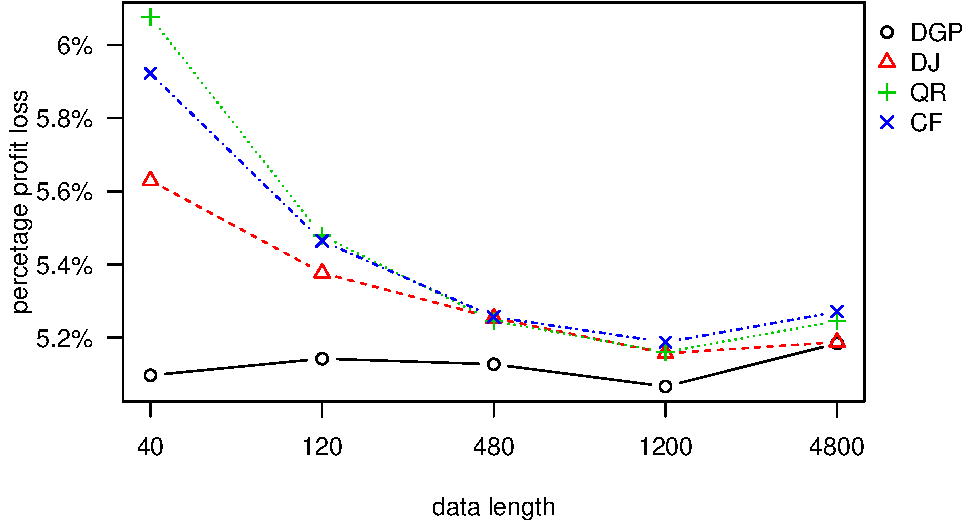
\includegraphics{linear-norm-plot_files/figure-latex/ppl0.3-1.pdf}
\label{fig:ppl0.3}
\end{figure}

\begin{figure}[ht]
\centering
\caption{Service level vs. data size at 0.3 target service level}
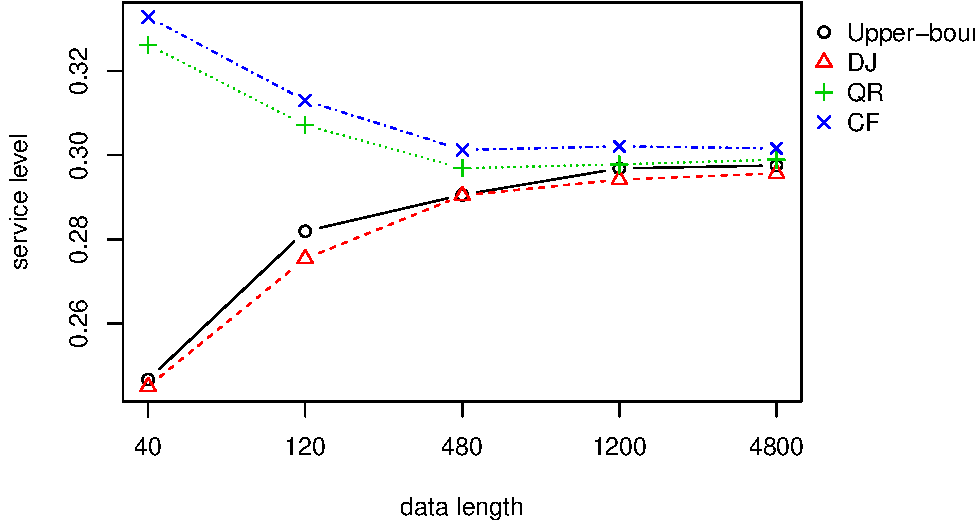
\includegraphics{linear-norm-plot_files/figure-latex/sl-3.pdf}
\label{fig:sl0.3}
\end{figure}

Figure \ref{fig:sl0.3} represents the average SL, i.e., the proportion of iterations in which the demand was satisfied in the simulation.
We see that all four methods converge to the desired target of 0.3 as the sample size grows. Interestingly, DGP and DJ approach the target from below, while PM and QR approach it from above. A possible explanation is as follows. In the first phase of DGP and DJ, the estimated variance tends to be larger than the true variance when the sample size is small. This causes the estimated order quantities in simulation often to be more spread than it should be, and thus leads to low SL. On the other hand, the integrated methods take the underage and overage costs into account. For the given cost parameters, over-stocking is less costly than under-stocking, as a result the methods achieve higher service level than needed.

Figure \ref{fig:fr0.3} represents the average FR. As one might expect, the average fill rate gets better as sample size grows in all methods. 


\begin{figure}[ht]
\centering
\caption{Fill rate vs. data size at 0.3 target service level}
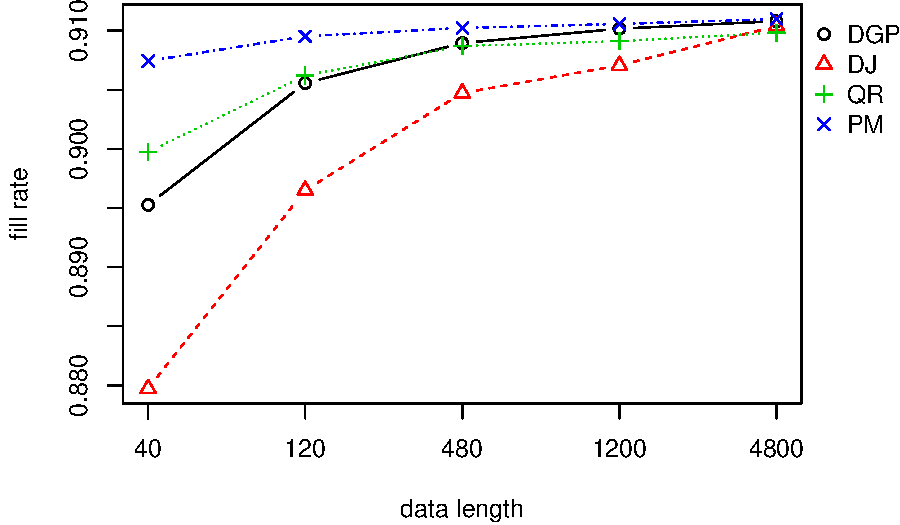
\includegraphics{linear-norm-plot_files/figure-latex/fr-3.pdf}
\label{fig:fr0.3}
\end{figure}

Next, we explore whether the target service level has a significant effect on the performance of the methods. Specifically, we considered the following two alternative parameter settings:
\begin{itemize}
    \item $p=20$, $v=8$, $c_h=-3$, $c_s=-7$
    \item $p=20$, $v=8$, $c_h=3$, $c_s=7$.
\end{itemize}
One can check that the corresponding pairs $\big( c_u,c_o \big)$ are $(5,5)$ and $(19,11)$, respectively. Thus, the target service level evaluates to $0.5$ and $0.63$, respectively.

The relevant data is given in Tables \ref{tab:level_effect40} and \ref{tab:level_effect4800}, for the cases $s=40$
and $s=4800$, respectively. Generally speaking, the picture is similar, regardless of the target service level. An exception is that the PPL is particularly high for all the methods when the target service level is 0.63. This is probably due to the relatively large overage and underage costs in that case.

\begin{table}
\caption{Target service level effect with $s=40$}
\label{tab:level_effect40}
\centering
\resizebox{\linewidth}{!}{
\begin{tabular}{ccccccccccccc}
\toprule
\multicolumn{1}{c}{\textbf{ }} & \multicolumn{4}{c}{\textbf{Percentage profit loss}} & \multicolumn{4}{c}{\textbf{Service level}} & \multicolumn{4}{c}{\textbf{Fill rate}} \\
\cmidrule(l{3pt}r{3pt}){2-5} \cmidrule(l{3pt}r{3pt}){6-9} \cmidrule(l{3pt}r{3pt}){10-13}
Target service level & DGP & disjoint & quantile & proposed & DGP & disjoint & quantile & proposed & DGP & disjoint & quantile & proposed\\
\midrule
0.5 & 5.0\% & 5.4\% & 5.4\% & 5.3\% & 0.50 & 0.44 & 0.50 & 0.50 & 95.2\% & 93.5\% & 94.7\% & 94.8\%\\
0.63 & 14.1\% & 15.2\% & 15.0\% & 14.8\% & 0.67 & 0.58 & 0.63 & 0.62 & 97.5\% & 95.8\% & 96.6\% & 96.6\%\\
0.3 & 5.0\% & 5.6\% & 5.6\% & 5.5\% & 0.25 & 0.25 & 0.31 & 0.31 & 89.7\% & 88.2\% & 90.6\% & 90.8\%\\
\bottomrule
\end{tabular}}
\end{table}

\begin{table}
\caption{Target service level effect with $s=4800$}
\label{tab:level_effect4800}
\centering
\resizebox{\linewidth}{!}{
\begin{tabular}{ccccccccccccc}
\toprule
\multicolumn{1}{c}{\textbf{ }} & \multicolumn{4}{c}{\textbf{Percentage profit loss}} & \multicolumn{4}{c}{\textbf{Service level}} & \multicolumn{4}{c}{\textbf{Fill rate}} \\
\cmidrule(l{3pt}r{3pt}){2-5} \cmidrule(l{3pt}r{3pt}){6-9} \cmidrule(l{3pt}r{3pt}){10-13}
Target service level & DGP & disjoint & quantile & proposed & DGP & disjoint & quantile & proposed & DGP & disjoint & quantile & proposed\\
\midrule
0.5 & 5.0\% & 5.0\% & 5.0\% & 5.0\% & 0.50 & 0.50 & 0.50 & 0.50 & 95.2\% & 95.2\% & 95.2\% & 95.2\%\\
0.63 & 14.0\% & 14.0\% & 14.1\% & 14.1\% & 0.63 & 0.63 & 0.63 & 0.63 & 97.0\% & 96.9\% & 96.9\% & 96.9\%\\
0.3 & 5.1\% & 5.1\% & 5.2\% & 5.2\% & 0.30 & 0.30 & 0.30 & 0.30 & 91.0\% & 90.9\% & 90.9\% & 91.0\%\\
\bottomrule
\end{tabular}}
\end{table}

\subsubsection{Nonlinear profit functions} \label{sub:exp2}

In this subsection, we examine the relative performance of the methods when applied to the NNV. As before, we assume that the DGP for the demands is an ARIMA $(1,0,0)(1,0,0)_4$ process, and the error term follows a normal distribution. We use the following nonlinear profit function \cite{KK18}:
\[
    \pi(Q,y)=
    \begin{cases}
        20y-8Q-4(Q-y)+5\E[\min \{(Q-y),u\}],& \text{if } Q\geq y\\
        20Q-8Q-0.01(y-Q)^2,& \text{if } Q< y,
    \end{cases}
\]
where $u\sim \mathcal{N}(30,5^2)$. Given that the target service level does not have a closed form in the NNV, one can use the technique mentioned in \cite{KK18}, or other numerical approaches, to verify that it approximates to 0.56.

Since the nonlinearity makes QR impossible to apply as we stated in Subsection \ref{sub:lit3}, we present results only for DJ and PM, together with the ``idealised" method based on the DGP.

Figure \ref{fig:non} shows the PPL and SL of each method, for each sample size. It is apparent that both DJ and PM methods perform well in terms of PPL, with very similar values for all sample sizes, but, as expected, they cannot outperform the DGP. However, the picture is very different with SL: the SL of the proposed method is very close to the the target service level even when the sample size is small. By contrast, the disjoint method needs more data to reach the target service level, and it approaches it from below. The reason is similar to the one we presented in Subsection \ref{sub:exp1}. 

Another thing to note is that with the increase of the sample size, the methods converge to the DGP values.

\begin{figure}[ht]
\centering
\caption{Performance vs. data size with nonlinear profit function}
\begin{subfigure}[b]{0.48\textwidth}
\centering
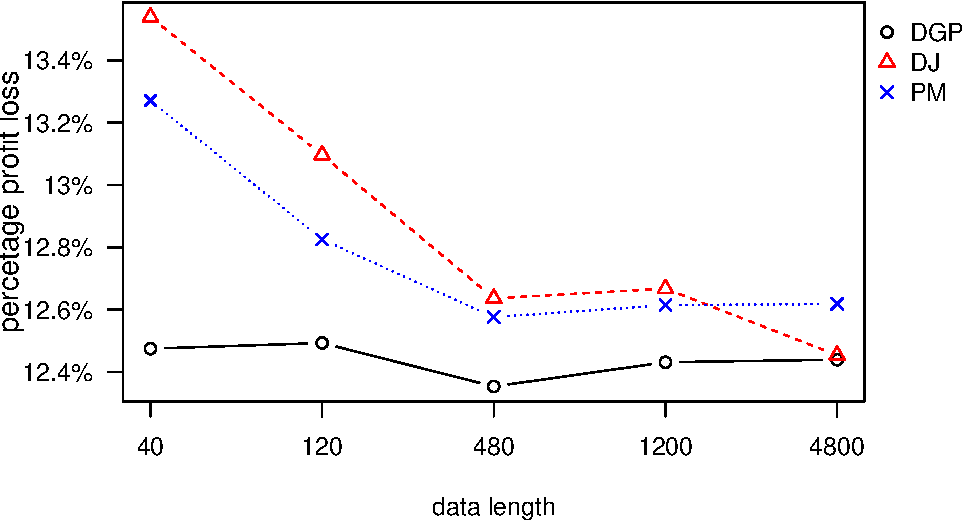
\includegraphics[width=\textwidth]{nonlinear-plot_files/figure-latex/ppl-1.pdf}
\caption{percentage profit loss vs. data size}
\end{subfigure}
\hfill
\begin{subfigure}[b]{0.48\textwidth}
\centering
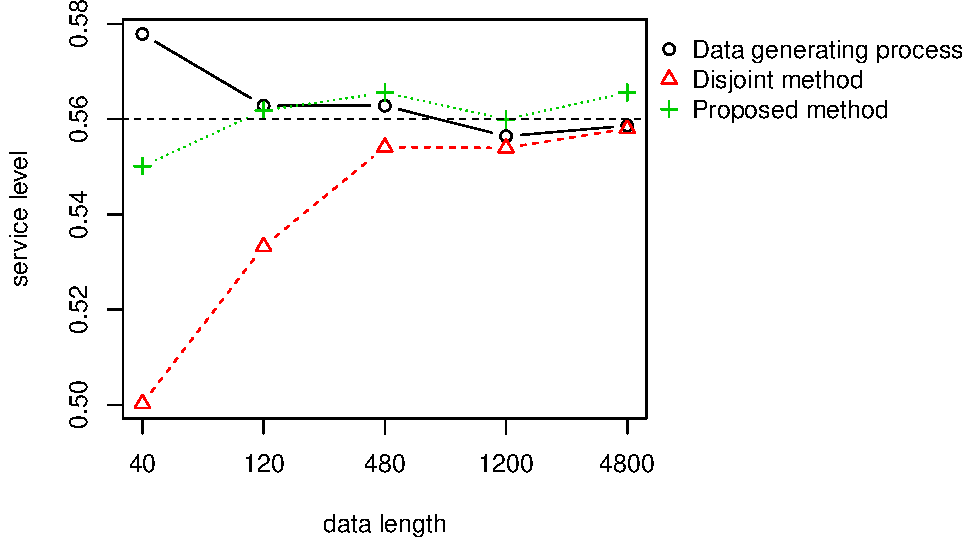
\includegraphics[width=\textwidth]{nonlinear-plot_files/figure-latex/sl-1.pdf}
\caption{service level vs. data size}
\end{subfigure}
\label{fig:non}
\end{figure}

We would like to stress that the proposed method does not need any complicated numerical optimisation or simulation methods to estimate the optimal order quantity. In addition, we have found that, for these instances, it typically required less computing time than the disjoint method. For example, only $\nicefrac{1}{10}$ amount of computing time is needed by using our proposed method comparing with DJ when $s=40$.
 
\subsection{The effect of misspecification} \label{sub:exp3}
\subsubsection{Linear case}

We now return to the linear case, and examine the effect of
\emph{model misspecification} on the performance of the disjoint method,
DJ, and our proposed method, PM, under the effect of misspecification. As we have shown the QR and PM are equivalent in linear NVP, we don't include QR here.

We first consider the situation in which our applied model is too simple.
In more detail, the data is still generated from a seasonal ARIMA $(1,0,0)(1,0,0)_4$ model, but we ignore seasonality when solving the NVP. In other words, when estimating the optimal order quantity, we use the incorrect assumption that the DGP is merely an AR$(1)$ process. %As in Subsection \ref{sub:exp1}, we assume that the error term of the demand follows a normal distribution, and we use the linear profit function with target service level $=0.3$.
\begin{figure}
\centering
\caption{Percentage profit loss vs. data size in misleading model}
\begin{subfigure}[b]{0.48\textwidth}
\centering
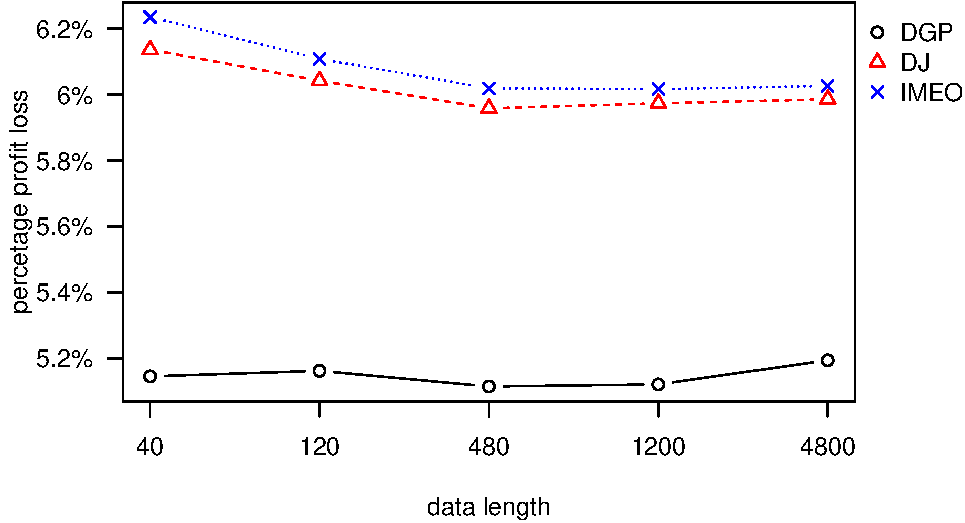
\includegraphics[width=\textwidth]{information-plot_files/figure-latex/AR(1)ppl-1.pdf}
\caption{misleading model AR$(1)$}
\end{subfigure}
\hfill
\begin{subfigure}[b]{0.48\textwidth}
\centering
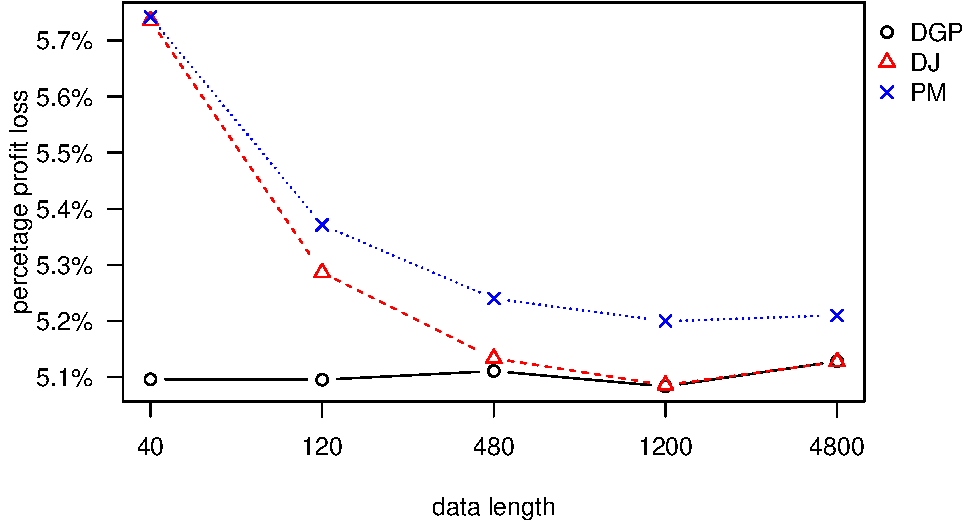
\includegraphics[width=\textwidth]{information-plot_files/figure-latex/SAR(3)(1)_4ppl-1.pdf}
\caption{misleading model ARIMA $(2,0,0)(1,0,0)_4$}
\end{subfigure}
\label{fig:mis}
\end{figure}

The percentage profit losses for this case can be seen in Figure
\ref{fig:mis} (a). By comparing with Figure \ref{fig:ppl0.3}, we see that the use of an incorrect model causes both DJ and PM to incur a small additional losses in profit irrespective of the sample size. These losses do not significantly improve as the number of data points increases, presumably because seasonality plays a key role when making one-step ahead forecasts. Interestingly, the performance of DJ and PM is similar, even though they are very different approaches. This could because the assumptions about the distribution of error term are correct.

\begin{figure}
\centering
\caption{Service level vs. data size in misleading model}
\begin{subfigure}[b]{0.48\textwidth}
\centering
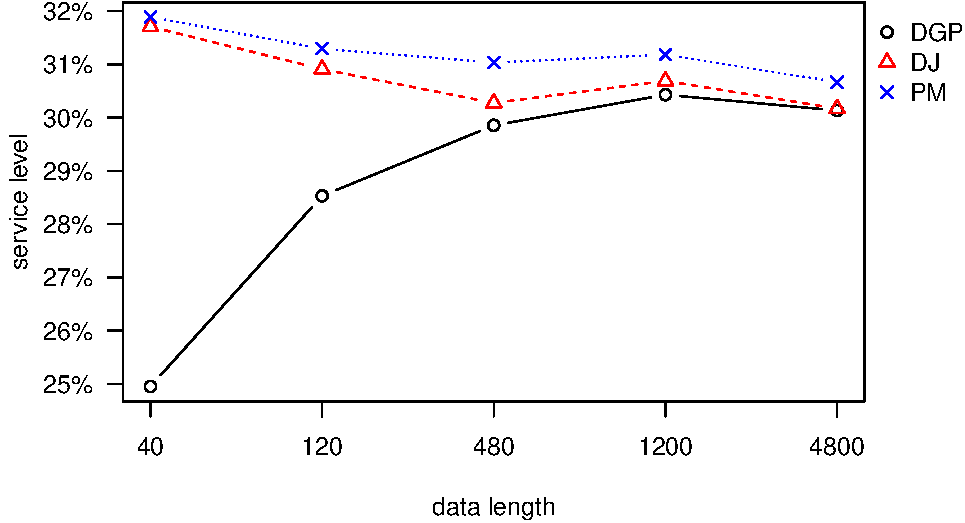
\includegraphics[width=\textwidth]{information-plot_files/figure-latex/AR(1)sl-1.pdf}
\caption{misleading model AR$(1)$}
\end{subfigure}
\hfill
\begin{subfigure}[b]{0.48\textwidth}
\centering
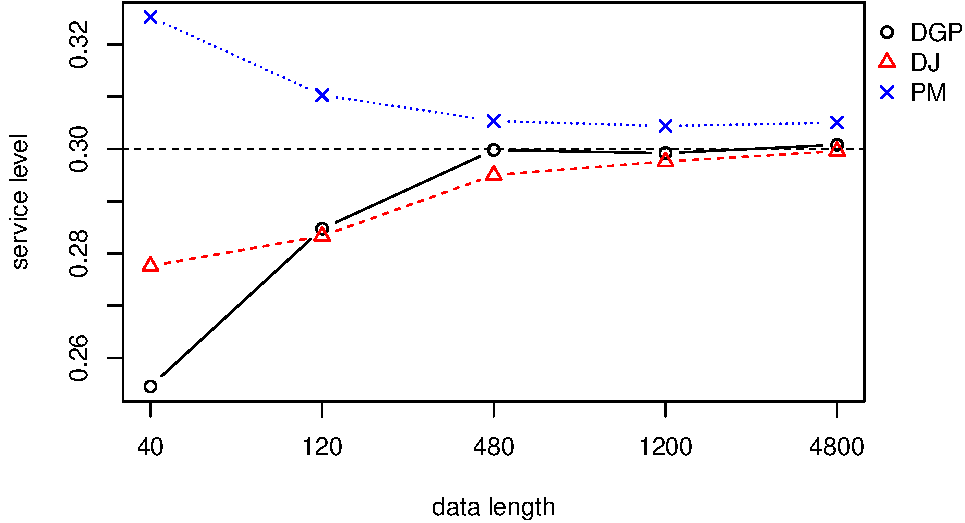
\includegraphics[width=\textwidth]{information-plot_files/figure-latex/SAR(3)(1)_4sl-1.pdf}
\caption{misleading model ARIMA $(2,0,0)(1,0,0)_4$}
\end{subfigure}
\label{fig:mis_sl}
\end{figure}

We also consider the situation where the applied model is overparameterised, ARIMA$(2,0,0)(1,0,0)_4$. The PPL for this case can be seen in Figure \ref{fig:mis} (b). Both DJ and PM incur a loss in profit, as before. Now, however, the loss decreases with the increase of the sample size. Indeed, closer inspection of the regression output revealed that, in both DJ and PM, the estimated value of the redundant model parameter tended to zero as the sample size increased. This can be explained by the well-known statistical phenomenon of redundant variables: they lead to less efficient estimates of parameters but do not incur the bias in the estimates as the effect of omitted variables typically does.

Besides, the service level for these two situations are presented in Figure \ref{fig:mis_sl}. The trend is similar to the one in Figure \ref{fig:sl0.3}.

Finally, we explore the effect on DJ and PM when the distribution of \emph{error term} is misspecified. In particular, we generate data using a modified version of our seasonal ARIMA$(1,0,0)(1,0,0)_4$ model, in which the error term follows a Laplace distribution with mean 0 and standard deviation 200. We remark that the Laplace distribution has ``fat tails", or, more formally, a higher kurtosis than the normal distribution. When estimating the optimal order quantity, however, we use the incorrect assumption that the error term follows a normal distribution.

The results for this scenario are presented in Figure \ref{fig:err}.
By comparing Figure \ref{fig:err}(a) with Figure \ref{fig:ppl0.3}, we see that the incorrect model of the noise leads only to a very small loss in profit for all the assessed methods. When we compare Figure \ref{fig:err}(b) with Figure \ref{fig:sl0.3}, the picture is rather different. As before, PM rapidly converges to the target service level (0.3) from above, while DJ achieves a lower than needed service level, and this drawback is not remedied by an increase in the sample size. A possible explanation is that our integrated approach works directly with the data, and is therefore, in a sense, ``non-parametric". This makes it more robust than the disjoint approach to deviations from normality.

\begin{figure}
\centering
\caption{Performance vs. data size with Laplace distributed error term}
\begin{subfigure}[b]{0.48\textwidth}
\centering
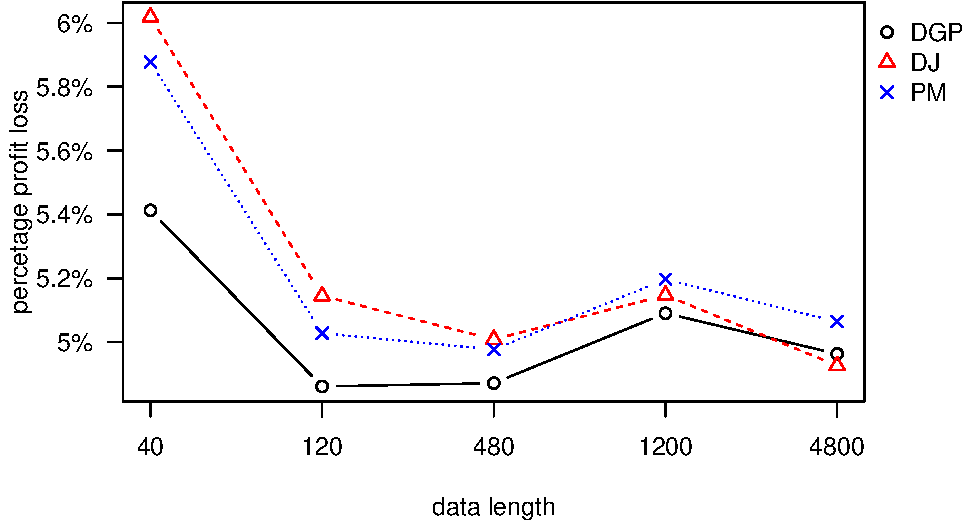
\includegraphics[width=\textwidth]{runif-plot_files/figure-latex/ppl-1.pdf}
\caption{percentage profit loss vs. data size}
\end{subfigure}
\hfill
\begin{subfigure}[b]{0.48\textwidth}
\centering
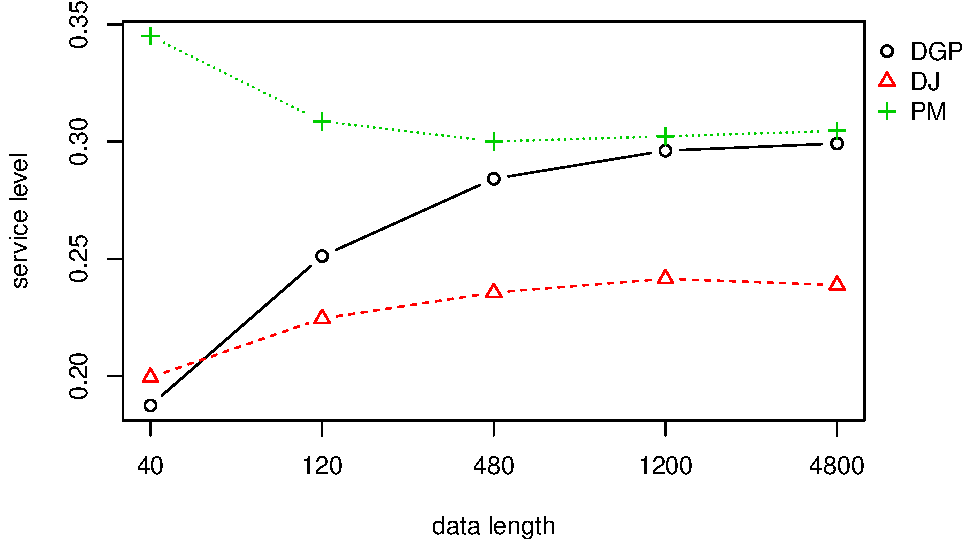
\includegraphics[width=\textwidth]{runif-plot_files/figure-latex/sl-1.pdf}
\caption{service level vs. data size}
\end{subfigure}
\label{fig:err}
\end{figure}

\subsubsection{Nonlinear case}


\section{Concluding Remarks} \label{se:end}

Newsvendor problem (NVP) is one of the most popular stochastic optimisation problems. It has different forms and can be typically solved either using a disjoint or integrated approaches. In this paper, we present the framework of a new integrated approach to NVP. The method is flexible, and doesn't make assumptions about the demand distribution, reducing the gap between the demand and the orders.%It could generate stable outcomes even in the case we possess misleading information or make wrong assumptions.
It is easy to understand and can be applied to wide variety of forecasting models.

We show analytically that the proposed approach is equivalent to quantile regression in simple linear cases of NVP, which makes the estimates of parameters of models in this case consistent, efficient and asymptotically follow normal distribution.

We then compare the performance of the proposed method with conventional disjoint method and quantile regression in several simulation experiments, considering the situations, when the demand forecasting model is correctly specified and when it is wrong. We find that in the former case the proposed method performs similar to the quantile regression and to the disjoint method in classic NVP in terms of the percentage profit loss, service level and fill rate. When considering the latter case, the proposed method performs in generally robustly, outperforming the disjoint method in some cases of model misspecification in terms of service level, and performing similar in terms of other error measures.

Furthermore, we have tested the methods in the case of nonlinear NVP, and found that the proposed method performs at least as good as the disjoint one in terms of percentage profit loss. However, it achieved the service level closer to the target one even on small samples, something that the disjoint method was not capable of doing in the same situation.

While this paper focused on a specific ARIMA model, we expect that the results could be generalised to such models as regression and ETS. However, we have not yet considered the cases, when the model family is incorrect, which could be considered as a direction for the future work. Another potential direction of future research is multi-product NVP, together with potential substitution effects between the products.

%%%%%%%%%%%%%%%%%%%%%%%%%%%%%%
\printbibliography

%%%%%%%%%%%%%%%%%%%%%%%%%%%%%%
\newpage
\begin{center}
{\bf\Large Appendices}
\end{center}

\appendix

\section{Scale and Shift Invariance}
\label{app:A}

For invariance with respect to scaling:
\[
    \begin{aligned}
        \hat{\boldsymbol{\beta}}(a\mathbf{y},\mathbf{X})
        &=\text{argmax}_{\boldsymbol{\beta}\in \mathbb{R}^{p+1}}\displaystyle\sum_{t=1}^s{\pi(\mathbf{x}_t^{\mathsf{T}}\boldsymbol{\beta},ay_t)}\\
        &=\text{argmin}_{\boldsymbol{\beta}\in \mathbb{R}^{p+1}}\displaystyle\sum_{t=1}^s{\{c_o[\mathbf{x}_t^{\mathsf{T}}\boldsymbol{\beta}-ay_t]^{+}+c_u[ay_t-\mathbf{x}_t^{\mathsf{T}}\boldsymbol{\beta}]^{+}\}}\\
        &=\text{argmax}_{\boldsymbol{\beta}\in \mathbb{R}^{p+1}}\displaystyle\sum_{t=1}^s{\pi\left(\mathbf{x}_t^{\mathsf{T}}\frac{\boldsymbol{\beta}}{a},y_t\right)}\\
        &=a\hat{\boldsymbol{\beta}}(\mathbf{y},\mathbf{X}).
    \end{aligned}
\]

\noindent
For invariance with respect to shifting:
\[
    \begin{aligned}
        &\hat{\boldsymbol{\beta}}(\mathbf{y}+\mathbf{X}\gamma,\mathbf{X})\\
        &\quad=\text{argmax}_{\boldsymbol{\beta}\in \mathbb{R}^{p+1}}\displaystyle\sum_{t=1}^s{\pi(\mathbf{x}_t^{\mathsf{T}}\boldsymbol{\beta},y_t+\mathbf{x}_t^{\mathsf{T}}\gamma)}\\
        &\quad=\text{argmin}_{\boldsymbol{\beta}\in \mathbb{R}^{p+1}}\displaystyle\sum_{t=1}^s{\{c_o[\mathbf{x}_t^{\mathsf{T}}\boldsymbol{\beta}-y_t-\mathbf{x}_t^{\mathsf{T}}\gamma]^{+}+c_u[y_t+\mathbf{x}_t^{\mathsf{T}}\gamma-\mathbf{x}_t^{\mathsf{T}}\boldsymbol{\beta}]^{+}\}}\\
        &\quad=\text{argmax}_{\boldsymbol{\beta}\in \mathbb{R}^{p+1}}\displaystyle\sum_{t=1}^s{\pi[\mathbf{x}_t^{\mathsf{T}}(\boldsymbol{\beta}-\gamma),y_t]}\\
        &\quad=\hat{\boldsymbol{\beta}}(\mathbf{y},\mathbf{X})+\gamma.
    \end{aligned}
\]

\section{Invariance under Reparameterization}
\label{app:B}

Define
    \[
        \mathbf{D}=\mathbf{X}A
        =\begin{pmatrix}
            \mathbf{d}_1^{\mathsf{T}}\\
            \mathbf{d}_2^{\mathsf{T}}\\
            \vdots\\
            \mathbf{d}_s^{\mathsf{T}}
        \end{pmatrix}
        =\begin{pmatrix}
            \mathbf{x}_{1}^{\mathsf{T}}\mathbf{a}^1&\mathbf{x}_1^{\mathsf{T}}\mathbf{a}^2&\cdots &\mathbf{x}_1^{\mathsf{T}}\mathbf{a}^{p+1}\\
            \mathbf{x}_2^{\mathsf{T}}\mathbf{a}^1&\mathbf{x}_2^{\mathsf{T}}\mathbf{a}^2&\cdots &\mathbf{x}_2^{\mathsf{T}}\mathbf{a}^{p+1}\\
            \vdots &\vdots &\ddots &\vdots \\
            \mathbf{x}_s^{\mathsf{T}}\mathbf{a}^1&\mathbf{x}_s^{\mathsf{T}}\mathbf{a}^2&\cdots &\mathbf{x}_s^{\mathsf{T}}\mathbf{a}^{p+1}
        \end{pmatrix},
    \]
    where $\mathbf{a}^n$ is the $n$th column of matrix $A$. We have
    \[
        \begin{aligned}
            &\hat{\boldsymbol{\beta}}(\mathbf{y},\mathbf{X}A)\\
            &\quad=\text{argmax}_{\boldsymbol{\beta}\in \mathbb{R}^{p+1}}\displaystyle\sum_{t=1}^s{\pi(\mathbf{d}_t^{\mathsf{T}}\boldsymbol{\beta},y_t)}\\
            &\quad=\text{argmin}_{\boldsymbol{\beta}\in \mathbb{R}^{p+1}}\displaystyle\sum_{t=1}^s{\{c_o[\mathbf{d}_t^{\mathsf{T}}\boldsymbol{\beta}-y_t]^{+}+c_u[y_t-\mathbf{d}_t^{\mathsf{T}}\boldsymbol{\beta}]^{+}\}}.
        \end{aligned}
    \]
    Note that
    \[
        \begin{aligned}
            \mathbf{d}_t^{\mathsf{T}}\boldsymbol{\beta}
            &=\displaystyle\sum_{n=1}^{p+1}\mathbf{x}_t^{\mathsf{T}}\mathbf{a}^n\beta_n\\
            &=\displaystyle\sum_{n=1}^{p+1}\displaystyle\sum_{m=1}^{p+1}x_{tm}a_{mn}\beta_n\\
            &=\displaystyle\sum_{m=1}^{p+1}x_{tm}\mathbf{a}_m^{\mathsf{T}}\boldsymbol{\beta}\\
            &=\mathbf{x}_t^{\mathsf{T}}A\boldsymbol{\beta},
        \end{aligned}
    \]
    where $a_{mn}$ is the element at $m$th row and $n$th column of $A$.
    From this, we have:
    \[
        \begin{aligned}
            &\hat{\boldsymbol{\beta}}(\mathbf{y},\mathbf{X}A)\\
            &\quad=\text{argmin}_{\boldsymbol{\beta}\in \mathbb{R}^{p+1}}\displaystyle\sum_{t=1}^s{\left\{c_o\left[\mathbf{x}_t^{\mathsf{T}}A\boldsymbol{\beta}-y_t\right]^{+}+c_u\left[y_t-\mathbf{x}_t^{\mathsf{T}}A\boldsymbol{\beta}\right]^{+}\right\}}\\
            &\quad=\text{argmax}_{\boldsymbol{\beta}\in \mathbb{R}^{p+1}}\displaystyle\sum_{t=1}^s{\pi(\mathbf{x}_t^{\mathsf{T}}A\boldsymbol{\beta},y_t)}\\
            &\quad=A^{-1}\hat{\boldsymbol{\beta}}(\mathbf{y},\mathbf{X}).
        \end{aligned}
    \]
    
\section{Equivalence to Quantile Regression}
\label{app:C}
Here, we show that the loss function used in the proposed method is transformable to the typical loss function of quantile regression. In quantile regression, the loss function is defined as \cite{KH01}:
\[
    \hat{\boldsymbol{\beta}}=\text{argmin}_{\boldsymbol{\beta}\in \mathbb{R}^{p+1}}\displaystyle\sum_{t=1}^s\rho_{\tau}(y_t-\mathbf{x}_t^{\mathsf{T}}\boldsymbol{\beta}),
\]
where $\displaystyle \rho_{\tau}(u)=u(\tau-\mathbb{I}_{(u<0)})$, and $\mathbb{I}$ is an indicator function. Thus, all we need to do is to prove that:
\[
    \text{max}\displaystyle\sum_{t=1}^s{\pi(\mathbf{x}_t^{\mathsf{T}}\boldsymbol{\beta},y_t)}=\text{min}\displaystyle\sum_{t=1}^s\rho_{\tau}(y_t-\mathbf{x}_t^{\mathsf{T}}\boldsymbol{\beta}).
\]
We have:
\[
    \min[a,b]=a-[a-b]^+,
\]
and
\[
    a-b=[a-b]^+-[b-a]^+.
\]
We can transform:
\[
    \begin{aligned}
        \pi(\mathbf{x}_t^{\mathsf{T}}\boldsymbol{\beta},y_t)
        &=p\min[\mathbf{x}_t^{\mathsf{T}}\boldsymbol{\beta},y_t]-v\mathbf{x}_t^{\mathsf{T}}\boldsymbol{\beta}-c_h[\mathbf{x}_t^{\mathsf{T}}\boldsymbol{\beta}-y_t]^+-c_s[y_t-\mathbf{x}_t^{\mathsf{T}}\boldsymbol{\beta}]^+\\
        &=p\{\mathbf{x}_t^{\mathsf{T}}\boldsymbol{\beta}-[\mathbf{x}_t^{\mathsf{T}}\boldsymbol{\beta}-y_t]^+\}-v\mathbf{x}_t^{\mathsf{T}}\boldsymbol{\beta}-c_h[\mathbf{x}_t^{\mathsf{T}}\boldsymbol{\beta}-y_t]^+-c_s[y_t-\mathbf{x}_t^{\mathsf{T}}\boldsymbol{\beta}]^+\\
        &=(p-v)\mathbf{x}_t^{\mathsf{T}}\boldsymbol{\beta}-(c_h+p)[\mathbf{x}_t^{\mathsf{T}}\boldsymbol{\beta}-y_t]^+-c_s[y_t-\mathbf{x}_t^{\mathsf{T}}\boldsymbol{\beta}]^+.
    \end{aligned}
\]
Therefore, we have (since $y_t$ is fixed):
\[
    \begin{aligned}
        &\text{max}\displaystyle\sum_{t=1}^s{\pi(\mathbf{x}_t^{\mathsf{T}}\boldsymbol{\beta},y_t)}\\
        &\quad=\text{max}\displaystyle\sum_{t=1}^s\{(p-v)\mathbf{x}_t^{\mathsf{T}}\boldsymbol{\beta}-(c_h+p)[\mathbf{x}_t^{\mathsf{T}}\boldsymbol{\beta}-y_t]^+-c_s[y_t-\mathbf{x}_t^{\mathsf{T}}\boldsymbol{\beta}]^+\}\\
        &\quad=\text{max}\displaystyle\sum_{t=1}^s\{(p-v)[\mathbf{x}_t^{\mathsf{T}}\boldsymbol{\beta}-y_t]-(c_h+p)[\mathbf{x}_t^{\mathsf{T}}\boldsymbol{\beta}-y_t]^+-c_s[y_t-\mathbf{x}_t^{\mathsf{T}}\boldsymbol{\beta}]^+\}\\
        &\quad=\text{max}\displaystyle\sum_{t=1}^s\{(p-v)[\mathbf{x}_t^{\mathsf{T}}\boldsymbol{\beta}-y_t]^+-(p-v)[y_t-\mathbf{x}_t^{\mathsf{T}}\boldsymbol{\beta}]^+\\
        &\qquad-(c_h+p)[\mathbf{x}_t^{\mathsf{T}}\boldsymbol{\beta}-y_t]^+-c_s[y_t-\mathbf{x}_t^{\mathsf{T}}\boldsymbol{\beta}]^+\}\\
        &\quad=\text{min}\displaystyle\sum_{t=1}^s\{(v+c_h)[\mathbf{x}_t^{\mathsf{T}}\boldsymbol{\beta}-y_t]^++(p-v+c_s)[y_t-\mathbf{x}_t^{\mathsf{T}}\boldsymbol{\beta}]^+\}\\
        &\quad=\text{min}\displaystyle\sum_{t=1}^s\{c_o[\mathbf{x}_t^{\mathsf{T}}\boldsymbol{\beta}-y_t]^++c_u[y_t-\mathbf{x}_t^{\mathsf{T}}\boldsymbol{\beta}]^+\}.
    \end{aligned}
\]
By setting $\tau=\nicefrac{c_u}{(c_o+c_u)}$, we have:
\[
    \text{max}\displaystyle\sum_{t=1}^s{\pi(\mathbf{x}_t^{\mathsf{T}}\boldsymbol{\beta},y_t)}=\text{min}\displaystyle\sum_{t=1}^s\{(1-\tau)[\mathbf{x}_t^{\mathsf{T}}\boldsymbol{\beta}-y_t]^++\tau[y_t-\mathbf{x}_t^{\mathsf{T}}\boldsymbol{\beta}]^+\}=\text{min}\displaystyle\sum_{t=1}^s\rho_{\tau}(y_t-\mathbf{x}_t^{\mathsf{T}}\boldsymbol{\beta}).
\]
\end{document}